\chapter{Project Management}
\section{Project Management}
Prima di introdurre il \textbf{Project Management} è necessario definire cosa si intende per \textbf{progetto}. Esistono diverse definizioni:

\begin{itemize}
    \item secondo il \textbf{PMI (Project Management Institute)}, un progetto è un'iniziativa temporanea intrapresa per creare 
    un prodotto o un servizio unico;
    \item secondo l'\textbf{HBS -- Manuale di Project Management}, un progetto è una serie unica di attività volte a produrre un 
    risultato definito, caratterizzata da una precisa data di inizio e di fine e da una determinata allocazione di risorse;
    \item secondo \textbf{R.D. Archibald}, un progetto è un'impresa complessa e unica, di durata predeterminata, finalizzata al raggiungimento 
    di un obiettivo chiaro e predefinito attraverso un processo continuo di pianificazione e controllo delle risorse, nel rispetto dei vincoli di costi, tempi e qualità.
\end{itemize}
\begin{figure}[H]
    \centering  
    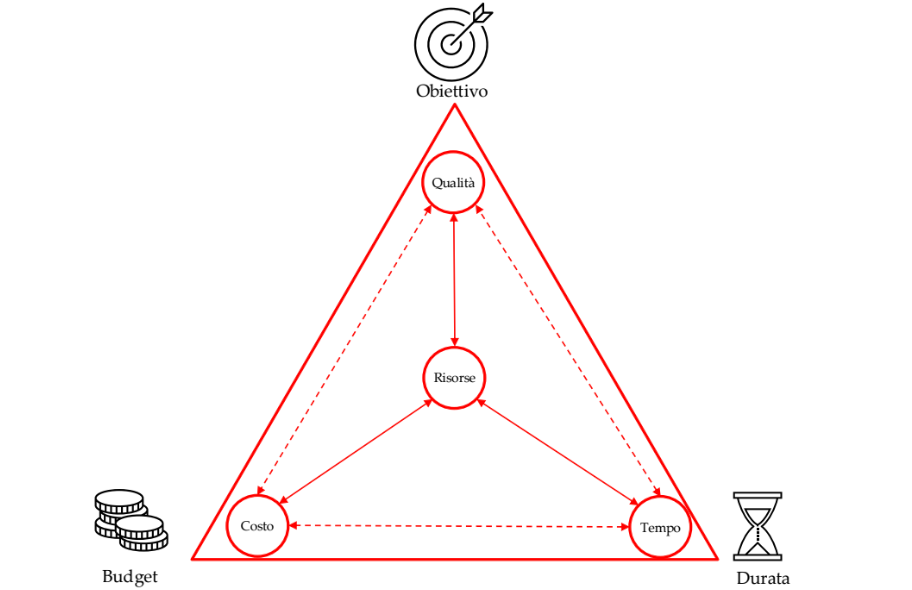
\includegraphics[width=0.9\linewidth]{../images/Piramide.png}
    \caption{Piramide del Project Management}
    %\label{label}
\end{figure}

\noindent In sintesi, un \textbf{progetto} è un insieme di attività complesse e interrelate, finalizzate al raggiungimento di un obiettivo ben definito. Tale obiettivo 
viene raggiunto attraverso sforzi coordinati e sinergici, entro un periodo di tempo prestabilito e utilizzando una quantità definita di risorse umane e finanziarie.

\noindent Le principali variabili da gestire all'interno di un progetto sono:
\begin{enumerate}
    \item \textbf{Qualità} $\rightarrow$ livello qualitativo dell'obiettivo e dei risultati del progetto;
    \item \textbf{Tempi} $\rightarrow$ durata del progetto e rispetto delle scadenze stabilite;
    \item \textbf{Costi} $\rightarrow$ risorse economiche necessarie per realizzare il progetto;
    \item \textbf{Risorse} $\rightarrow$ risorse umane, finanziarie e materiali disponibili, che costituiscono 
    dei vincoli per la realizzazione del progetto.
\end{enumerate}

\noindent Il \textbf{Project Management} consiste quindi nell'insieme delle attività di pianificazione, organizzazione, coordinamento 
e controllo necessarie per raggiungere gli obiettivi di un progetto rispettando i vincoli stabiliti.
\begin{figure}[H]
    \centering  
    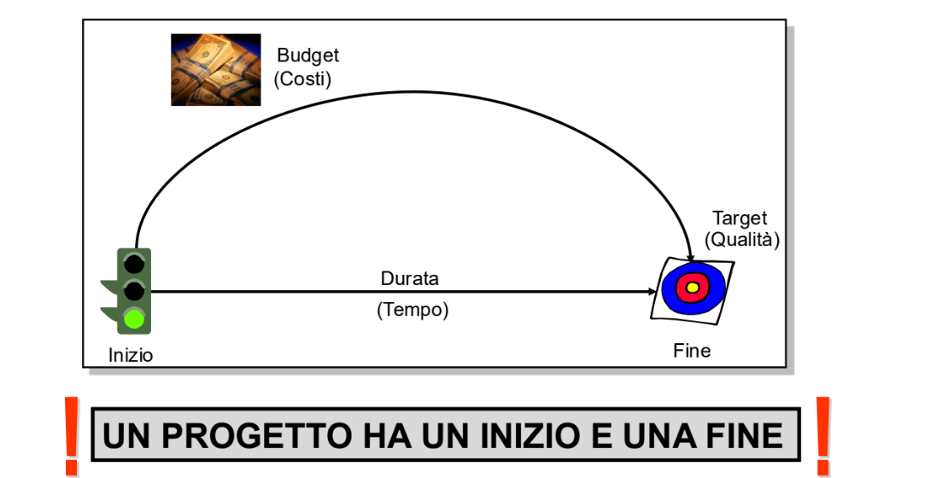
\includegraphics[width=0.9\linewidth]{../images/ERFUNZIO.png}
    %\label{label}
\end{figure}
\subsection{Operations Management e Project Management}

Le attività svolte all'interno di un'organizzazione possono essere suddivise in due categorie principali:
\begin{itemize}
    \item \textbf{Attività di routine} $\rightarrow$ la loro gestione prende il nome di \textbf{Operations Management (OM)};
    \item \textbf{Attività di cambiamento o innovazione} $\rightarrow$ la loro gestione prende il nome di \textbf{Project Management (PM)}.
\end{itemize}

\noindent Le prestazioni operative dell'Operations Management e del Project Management possono essere rappresentate graficamente come segue:
\begin{figure}[H]
    \centering
    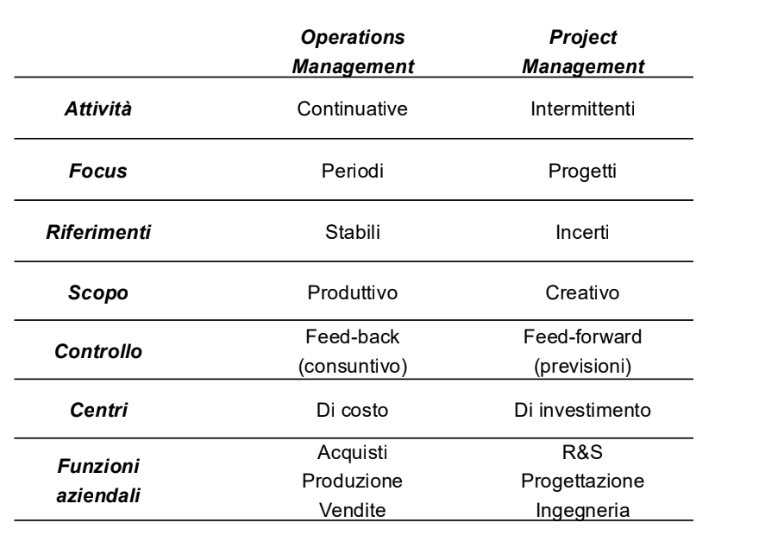
\includegraphics[width=0.6\linewidth]{../images/DIFFE OP PJ.png}
    \caption{Operations Management e Project Management}
\end{figure}

\noindent La separazione tra le due tipologie di attività, tuttavia, non è sempre così netta:
\begin{itemize}
    \item l'\textbf{Operations Management} deve essere in grado di rispondere anche a imprevisti e situazioni di incertezza;
    \item il \textbf{Project Management} cerca, quando possibile, di standardizzare attività che per loro natura sono uniche e non ripetitive.
\end{itemize}

\noindent Una delle principali differenze riguarda la durata delle attività. Il \textbf{Project Management è temporaneo}: ogni progetto possiede una data di inizio e una data di fine. L'\textbf{Operations Management}, invece, riguarda attività continuative e mira a garantire una produzione o un'erogazione di servizi il più possibile costante.

\noindent Le differenze principali possono essere riassunte come segue:
\begin{itemize}
    \item \textbf{Operations Management} $\rightarrow$ presenta riferimenti relativamente stabili, si basa su attività ripetitive e 
    dispone generalmente di dati storici. Il controllo riguarda sia il corretto svolgimento delle attività di routine sia il raggiungimento dei risultati previsti;
    \item \textbf{Project Management} $\rightarrow$ opera in condizioni caratterizzate da maggiore unicità e incertezza. 
    Il controllo viene effettuato sia \textit{in itinere}, durante lo svolgimento del progetto, sia \textit{ex post}, verificando i risultati ottenuti rispetto alle previsioni iniziali.
\end{itemize}

\subsection{Caratteristiche dei progetti}
Ogni progetto è \textbf{unico} e presenta caratteristiche differenti rispetto agli altri progetti. In particolare, possono variare:
\begin{itemize}
    \item obiettivi;
    \item durata;
    \item risorse finanziarie e umane;
    \item specificità dei piani;
    \item governance e organizzazione.
\end{itemize}

\subsection{Ambiti applicativi del Project Management}
I principali ambiti di applicazione del Project Management sono:
\begin{enumerate}
    \item \textbf{Progettazione e sviluppo di prodotti e servizi} $\rightarrow$ realizzazione di nuovi prodotti o 
    servizi oppure miglioramento di quelli già esistenti;
    \item \textbf{Gestione delle commesse} $\rightarrow$ realizzazione di attività sulla base di specifiche 
    richieste del committente;
    \item \textbf{Progettazione e miglioramento dei processi organizzativi} $\rightarrow$ introduzione di cambiamenti 
    finalizzati a rendere più efficaci ed efficienti i processi dell'organizzazione;
    \item \textbf{Ricerca pubblica e cooperazione internazionale} $\rightarrow$ gestione di progetti di ricerca, sviluppo e collaborazione tra 
    organizzazioni e Paesi differenti.
\end{enumerate}
\begin{figure}[H]
    \centering  
    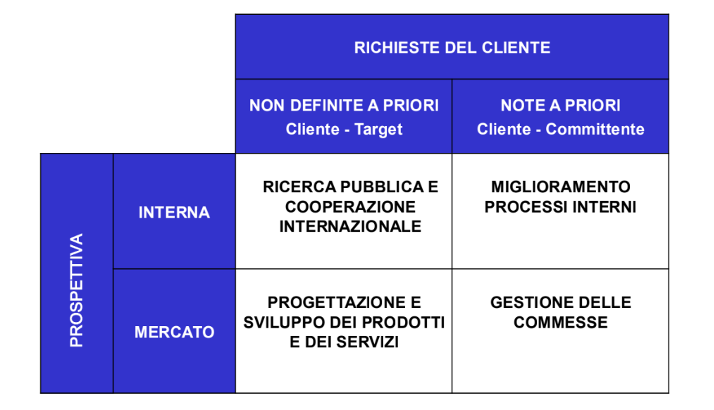
\includegraphics[width=0.5\linewidth]{../images/AMBI.png}
    \caption{caption}
    %\label{label}
\end{figure}
\subsection{Fattori critici di successo}
I \textbf{fattori critici di successo} rappresentano gli elementi che possono influenzare significativamente il raggiungimento degli obiettivi di un progetto.

\noindent Tra i principali troviamo:
\begin{enumerate}
    \item \textbf{Partecipazione e supporto del top management};
    \item \textbf{Competenze del Project Manager e del team di progetto};
    \item \textbf{Attuazione di strategie innovative};
    \item \textbf{Fattori interni}, tra cui:
    \begin{enumerate}
        \item cultura aziendale;
        \item struttura organizzativa;
        \item infrastrutture tecniche;
        \item direttive, procedure e documentazione standardizzata di Project Management;
        \item disponibilità di risorse umane;
        \item presenza di un \textbf{Project Management Information System (PMIS)};
        \item presenza di database contenenti informazioni sui progetti precedenti.
    \end{enumerate}
    \item \textbf{Fattori esterni} $\rightarrow$ elementi non direttamente controllabili dall'organizzazione che possono influenzare l'andamento del progetto.
\end{enumerate}

\noindent Le possibili casistiche possono essere rappresentate graficamente:
\begin{figure}[H]
    \centering
    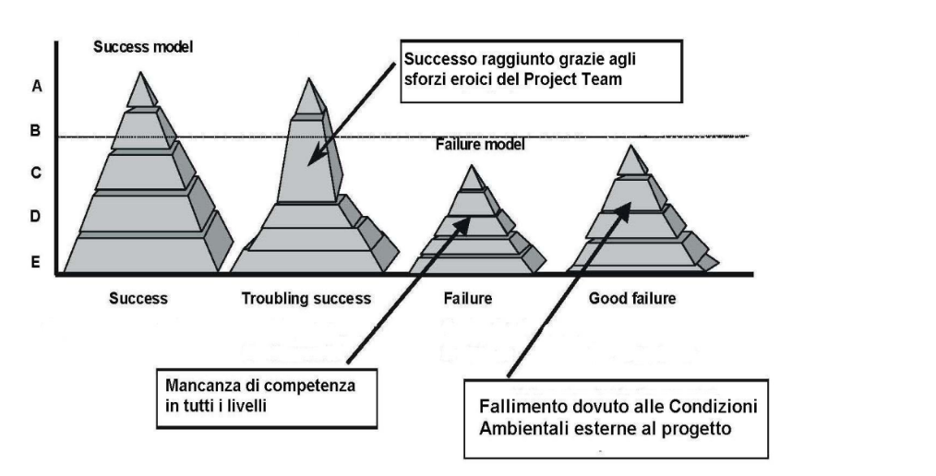
\includegraphics[width=0.9\linewidth]{../images/SUCCESSO.png}
    \caption{Possibili casistiche di successo e insuccesso di un progetto}
\end{figure}

\subsection{Principali cause di insuccesso}
Le principali cause che possono determinare l'insuccesso di un progetto sono:
\begin{itemize}
    \item \textbf{Missing Focus} $\rightarrow$ mancanza di obiettivi chiari e di una direzione precisa;
    \item \textbf{Content Issues} $\rightarrow$ problemi relativi ai contenuti, ai requisiti o alla definizione del progetto;
    \item \textbf{Skill Issues} $\rightarrow$ competenze insufficienti o non adeguate all'interno del team;
    \item \textbf{Execution Issues} $\rightarrow$ problemi nella fase di realizzazione ed esecuzione del progetto;
    \item \textbf{Unexplained Causes} $\rightarrow$ cause di insuccesso non chiaramente identificabili.
\end{itemize}

\noindent Per ridurre il rischio di insuccesso è necessario intervenire sulle diverse criticità attraverso una corretta pianificazione, 
un'attenta definizione degli obiettivi, l'assegnazione di risorse e competenze adeguate e un controllo continuo dell'avanzamento del progetto.
\subsection{Fattori per il successo di un progetto}
Per aumentare la probabilità di successo di un progetto è necessario intervenire su quattro aree principali:
\begin{itemize}
    \item \textbf{Strategia e stakeholder} $\rightarrow$ definire obiettivi chiari, un business case preciso, 
    coinvolgere i principali stakeholder, mantenere stabile lo scope del progetto e garantire il supporto del top management;
    \item \textbf{Tecnologia e contenuti} $\rightarrow$ utilizzare tecnologie standardizzate e consolidate e coinvolgere gli utenti 
    nella definizione della soluzione;
    \item \textbf{Team e competenze} $\rightarrow$ disporre di un Project Manager esperto, un team qualificato e motivato e un corretto 
    equilibrio tra risorse interne ed esterne;
    \item \textbf{Pratiche di Project Management} $\rightarrow$ effettuare stime e pianificazioni affidabili, garantire trasparenza sullo 
    stato del progetto e utilizzare metodologie e strumenti consolidati.
\end{itemize}

\noindent Il \textbf{successo del progetto} deriva quindi dalla combinazione di una strategia chiara, tecnologie adeguate, un team 
competente e una corretta applicazione delle pratiche di Project Management.

\begin{figure}[H]
    \centering  
    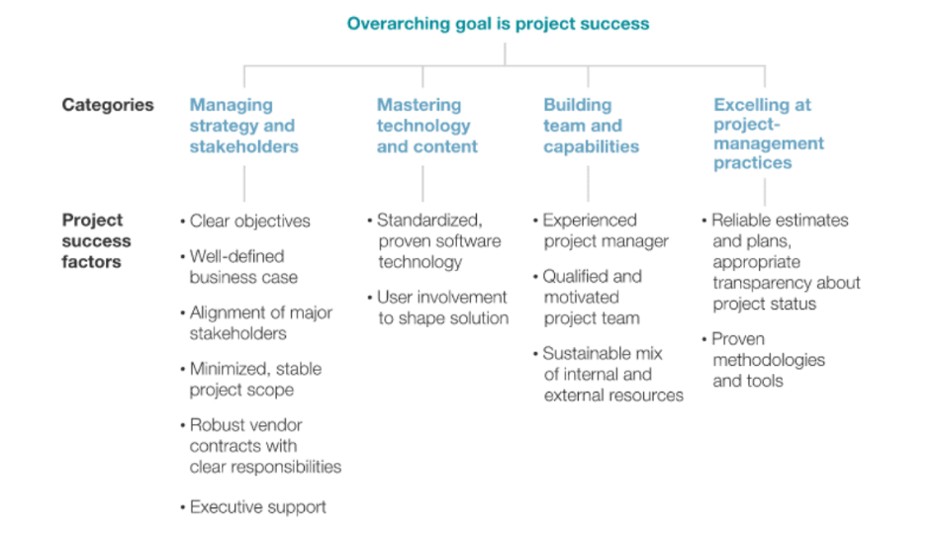
\includegraphics[width=0.9\linewidth]{../images/OLE.png}
    \caption{Obiettivi}
    %\label{label}
\end{figure}